\documentclass[conference]{IEEEtran}
\IEEEoverridecommandlockouts
% The preceding line is only needed to identify funding in the first footnote. If that is unneeded, please comment it out.
\usepackage{cite}
\usepackage{amsmath,amssymb,amsfonts}
\usepackage{algorithmic}
\usepackage{graphicx}
\usepackage{textcomp}
\usepackage{xcolor}

\usepackage{comment}

\def\BibTeX{{\rm B\kern-.05em{\sc i\kern-.025em b}\kern-.08em
    T\kern-.1667em\lower.7ex\hbox{E}\kern-.125emX}}








\usepackage{cite}
\usepackage{amsmath,amssymb,amsfonts}
\usepackage{graphicx}
\usepackage{booktabs}
\usepackage{textcomp}
\usepackage[hidelinks]{hyperref}
\usepackage{array}
\usepackage{comment}
\usepackage{tikz}
\usetikzlibrary{shapes.geometric,arrows.meta,positioning,calc}

% --- self-contained pseudocode -------------------------------------------
% Deliberately does not use algorithm/algpseudocode/algorithm2e: this way the
% paper compiles on any TeX installation without extra packages. `float` is
% part of every standard distribution.
\usepackage{float}
\floatstyle{plaintop}          % caption above the pseudocode, as is conventional
\newfloat{algorithm}{tbp}{loa}
\floatname{algorithm}{Algorithm}
\restylefloat{algorithm}
\newcounter{algline}
\newenvironment{pseudo}
  {\setcounter{algline}{0}\footnotesize
   \begin{list}{\scriptsize\arabic{algline}:}%
     {\usecounter{algline}%
      \setlength{\leftmargin}{1.7em}\setlength{\labelwidth}{1.2em}%
      \setlength{\labelsep}{0.5em}\setlength{\itemsep}{1pt}%
      \setlength{\parsep}{0pt}\setlength{\topsep}{3pt}%
      \setlength{\partopsep}{0pt}\raggedright}}
  {\end{list}}
\newcommand{\kw}[1]{\textbf{#1}}          % keyword
\newcommand{\pr}[1]{\textsc{#1}}          % procedure name
\newcommand{\IND}{\hspace*{1.2em}}        % one indent level
\newcommand{\cmt}[1]{{\itshape\,// #1}}   % comment

% --- revision highlighting -------------------------------------------------
% Marks text added in this revision, as requested by the reviewer. To produce a
% clean camera-ready, redefine \rev as \newcommand{\rev}[1]{#1} -- nothing else
% needs to change. \soulregister lets \hl survive the commands it would
% otherwise break on.
\usepackage{soul}
\usepackage{xcolor}
\sethlcolor{yellow}
\soulregister{\cite}{7}
\soulregister{\ref}{7}
\soulregister{\emph}{7}
\soulregister{\textit}{7}
\soulregister{\texttt}{7}
\soulregister{\NRecall}{7}
\soulregister{\NOpen}{7}
\soulregister{\NLogic}{7}
\soulregister{\VerifiedN}{7}
\soulregister{\ExcludedRows}{7}
\soulregister{\ExcludedReasons}{7}
\soulregister{\VerifiedDomains}{7}
\newcommand{\rev}[1]{\hl{#1}}
% Second revision round, in blue. Deliberately \textcolor rather than \hl:
% soul cannot span inline maths or nested marks, both of which occur below.
% For camera-ready, redefine both \rev and \revb as \newcommand{\x}[1]{#1}.
\newcommand{\revb}[1]{\textcolor{blue}{#1}}
\newcommand{\newrevb}{\textcolor{blue}{\scriptsize\bfseries [new in this revision]}}
% Third revision round: responses to the inference-time, benchmark-alignment,
% and near-ceiling-accuracy comments. For camera-ready, redefine \revg as
% \newcommand{\revg}[1]{#1}.
\definecolor{reviewgreen}{RGB}{0,128,0}
\newcommand{\revg}[1]{\textcolor{reviewgreen}{#1}}
% Marker for section headings and captions. soul's \hl cannot be used there:
% those are moving arguments and \hl breaks when LaTeX re-reads them. Use as
% \protect\newrev.
\newcommand{\newrev}{\colorbox{yellow}{\scriptsize\bfseries new in this revision}}
\graphicspath{{figs/}}

% Generated by make_numbers.py from the locked run artifacts.
% AUTO-GENERATED by make_numbers.py -- do not edit by hand.
% Sources (locked, read-only):
%   artifacts/locked_results/verified_v1_20260521_173612_CEST
%   artifacts/paper_handoff_20260603/off_system_eval_summary.csv

\newcommand{\AbstainShareLINC}{78}
\newcommand{\AbstainShareLogicLM}{3}
\newcommand{\AbstainShareLongCtx}{0}
\newcommand{\AccLINC}{94.88}
\newcommand{\AccLINCLogic}{95.36}
\newcommand{\AccLINCOpen}{91.62}
\newcommand{\AccLINCRecall}{95.45}
\newcommand{\AccLeastRuleLongCtx}{97.75}
\newcommand{\AccLogicLM}{96.99}
\newcommand{\AccLogicLMLogic}{93.62}
\newcommand{\AccLogicLMOpen}{97.82}
\newcommand{\AccLogicLMRecall}{99.96}
\newcommand{\AccLongCtx}{96.57}
\newcommand{\AccLongCtxLogic}{93.09}
\newcommand{\AccLongCtxOpen}{96.56}
\newcommand{\AccLongCtxRecall}{99.93}
\newcommand{\AccMostRuleLongCtx}{93.70}
\newcommand{\AccSys}{100.00}
\newcommand{\AccSysLogic}{100.00}
\newcommand{\AccSysOpen}{100.00}
\newcommand{\AccSysRecall}{100.00}
\newcommand{\BaseBestLogic}{95.36}
\newcommand{\BaseBestOpen}{97.82}
\newcommand{\BaseBestRecall}{99.96}
\newcommand{\BaseWorstLogic}{93.09}
\newcommand{\BaseWorstOpen}{91.62}
\newcommand{\BaseWorstRecall}{95.45}
\newcommand{\BestAtLogic}{LINC}
\newcommand{\BestAtOpen}{LogicLM}
\newcommand{\BestAtRecall}{LogicLM}
\newcommand{\CleanLINCLogic}{99.88}
\newcommand{\CleanLogicLMLogic}{99.39}
\newcommand{\CleanLongCtxLogic}{98.99}
\newcommand{\CompLogic}{1.00}
\newcommand{\CompMaxLogic}{1}
\newcommand{\CompMaxOpen}{6}
\newcommand{\CompMaxRecall}{7}
\newcommand{\CompOpen}{1.71}
\newcommand{\CompRecall}{1.02}
\newcommand{\DerivMax}{3}
\newcommand{\DerivMin}{1}
\newcommand{\DiscBaselineOnlyMax}{0}
\newcommand{\DiscLINCBaseOnly}{0}
\newcommand{\DiscLINCSysOnly}{321}
\newcommand{\DiscLogicLMBaseOnly}{0}
\newcommand{\DiscLogicLMSysOnly}{189}
\newcommand{\DiscLongCtxBaseOnly}{0}
\newcommand{\DiscLongCtxSysOnly}{215}
\newcommand{\DocCompoundPctOpen}{38}
\newcommand{\DocCompoundPctRec}{19}
\newcommand{\DocGoldCharsOpen}{29.8}
\newcommand{\DocGoldCharsRec}{19.5}
\newcommand{\DomainAgreeMin}{100}
\newcommand{\DomainLeastRule}{viessmann}
\newcommand{\DomainMostRule}{battery}
\newcommand{\DomainOrdering}{monotone}
\newcommand{\EmbedModel}{\texttt{all-MiniLM-L6-v2}}
\newcommand{\ErrLINC}{321}
\newcommand{\ErrLogicLM}{189}
\newcommand{\ErrLongCtx}{215}
\newcommand{\ErrSys}{0}
\newcommand{\ExcludedReasons}{8}
\newcommand{\ExcludedRows}{645}
\newcommand{\GenModel}{\texttt{gpt-4o-mini}}
\newcommand{\HeadroomLogic}{4.64}
\newcommand{\HeadroomOpen}{2.18}
\newcommand{\HeadroomOrdering}{increasing}
\newcommand{\HeadroomRecall}{0.04}
\newcommand{\McnExp}{56}
\newcommand{\MixedDoubleLabel}{0}
\newcommand{\MixedLogicNumeric}{0}
\newcommand{\MixedOpenNumeric}{0}
\newcommand{\MixedRecallMulti}{27}
\newcommand{\NDocSplit}{1{,}005}
\newcommand{\NLogic}{2{,}649}
\newcommand{\NOpen}{871}
\newcommand{\NOpenCompound}{325}
\newcommand{\NOpenDoc}{860}
\newcommand{\NRecall}{2{,}750}
\newcommand{\NRecallDoc}{145}
\newcommand{\NRecallKB}{2{,}594}
\newcommand{\NoRuleDiscLINC}{198}
\newcommand{\NoRuleDiscLogicLM}{20}
\newcommand{\NoRuleDiscLongCtx}{32}
\newcommand{\NoRuleLINC}{94.53}
\newcommand{\NoRuleLogicLM}{99.45}
\newcommand{\NoRuleLongCtx}{99.12}
\newcommand{\NoRuleN}{3{,}621}
\newcommand{\NoRuleRegressLINC}{0}
\newcommand{\NoRuleRegressLogicLM}{0}
\newcommand{\NoRuleRegressLongCtx}{0}
\newcommand{\NoRuleSys}{100.00}
\newcommand{\OffAbstainPrec}{0.998}
\newcommand{\OffAbstainRec}{1.000}
\newcommand{\OffAcc}{97.21}
\newcommand{\OffAccHi}{97.68}
\newcommand{\OffAccLo}{96.66}
\newcommand{\OffAurc}{0.025}
\newcommand{\OffCoverage}{73.0}
\newcommand{\OffEce}{0.021}
\newcommand{\OffEceHardest}{0.060}
\newcommand{\OffHardestAcc}{91.92}
\newcommand{\OffHardestCoverage}{38.0}
\newcommand{\OffHardestType}{sustainability}
\newcommand{\OffN}{4{,}021}
\newcommand{\OffSustCoverage}{38.0}
\newcommand{\OffTypes}{5}
\newcommand{\OpenAtomicLogicLM}{99.82}
\newcommand{\OpenAtomicLongCtx}{99.63}
\newcommand{\OpenCompoundLogicLM}{94.46}
\newcommand{\OpenCompoundLongCtx}{91.38}
\newcommand{\ScopeNarrow}{173}
\newcommand{\ShareLeastRule}{33.3}
\newcommand{\ShareMostRule}{53.9}
\newcommand{\SpreadLogic}{2.27}
\newcommand{\SpreadOpen}{6.20}
\newcommand{\SpreadOverall}{2.11}
\newcommand{\SpreadRecall}{4.51}
\newcommand{\SymFired}{2{,}649}
\newcommand{\SymFiredAcc}{100.00}
\newcommand{\SymFiredPct}{100}
\newcommand{\UnitRuleAgreement}{100}
\newcommand{\VerifiedDomains}{3}
\newcommand{\VerifiedN}{6{,}270}
\newcommand{\WorstAtLogic}{LongCtx}
\newcommand{\WorstAtOpen}{LINC}
\newcommand{\WorstAtRecall}{LINC}
















\begin{document}

\title{
%Finding Evidence Is Solved, Combining It Is Not:\\
A Fusion-Depth Analysis of Question Answering\\
over Digital Product Passports}

\author{\IEEEauthorblockN{A M Esfar E Alam* and Amir Taherkordi}
\IEEEauthorblockA{
%\textit{Department of Informatics} \\
\textit{University of Oslo, Norway} \\
\{aeturzo,amirhost\}@ifi.uio.no}
\and
\IEEEauthorblockN{Chenghua Lin}
\IEEEauthorblockA{
\textit{University of Manchester, UK} \\
chenghua.lin@manchester.ac.uk}}

\maketitle



\begin{abstract}
Digital Product Passport (DPP) question answering requires different levels of evidence fusion, from retrieving stated values to combining product evidence with external schema rules. This paper introduces a \emph{fusion-depth} perspective that categorizes questions as recall, open, or rule-governed according to their evidence requirements. We construct a benchmark of 6,270 verified questions across three industrial domains using a deterministic generation and verification procedure. Evaluation of long-context and neuro-symbolic approaches reveals clear depth-dependent trade-offs, with methods performing differently \revg{across fusion depths}. A depth-aware configuration that selectively engages retrieval, memory, and symbolic reasoning \revg{reaches the 100\% ceiling on this controlled, verified benchmark}, correcting baseline errors without losing correctly answered questions. On 4,021 queries from an unseen public product database, it achieves 97.21\% decision accuracy while appropriately reducing coverage when evidence is insufficient. These results show that adapting evidence fusion to question requirements improves the accuracy and reliability of DPP question answering.

\begin{comment}
Digital Product Passport (DPP) question answering must do more than locate
product information. Some questions need one stated value, some require
evidence from several parts of a record, and others require product evidence
to be combined with an external rule. Existing approaches usually apply one
reasoning strategy to all of these cases. Long-context models leave the
combination largely to the language model, while neuro-symbolic methods can
route every question through formal reasoning. We ask whether one strategy is
equally suitable across these different levels of evidence fusion.

We group questions by \emph{fusion depth}: recall questions require one stated
value, open questions require a compound value to be reproduced in full, and
rule-governed questions require a stated value to be combined with the schema
rules that classify it, so that the answer is entailed rather than stated. On
\VerifiedN{} verified questions across \VerifiedDomains{} industrial domains (battery,printer,heatpump),
the published configurations show a clear trade-off. Long-context and
Logic-LM reach \AccLongCtxRecall\% and \AccLogicLMRecall\% on recall questions
but fall to \AccLongCtxLogic\% and \AccLogicLMLogic\% on rule-governed
questions. LINC shows the opposite pattern, reaching \AccLINCLogic\% on
rule-governed questions but performing worst at the shallower depths. The
remaining accuracy gap to a perfect score grows from \HeadroomRecall{} points
for recall to \HeadroomOpen{} for open and \HeadroomLogic{} for rule-governed
questions.

A depth-aware configuration that applies symbolic validation only when needed
and abstains when the evidence is insufficient answers all \VerifiedN{}
verified questions correctly; no baseline correctly answers a question that
it misses. On \OffN{} queries from an unseen public product database, it
achieves \OffAcc\% decision accuracy while answering \OffCoverage\% of queries,
with a calibration error of \OffEce{}. These results suggest that evidence
fusion should match the needs of the question rather than applying the same
reasoning strategy uniformly.
\end{comment}
\end{abstract}

\begin{IEEEkeywords}
intelligent data fusion, digital product passport, question answering, selective prediction, large language model, long-context model, neuro-symbolic reasoning.
\end{IEEEkeywords}

% =====================================================================
\section{Introduction}
% =====================================================================

A Digital Product Passport, or DPP, is a structured record that describes a
product across its life. It can contain its materials, technical properties,
compliance evidence, repair information, environmental indicators, and
end-of-life instructions. European product policy is making DPPs an important
way to disclose such information~\cite{eu2024espr}. These records may be used
by auditors, regulators, manufacturers, and procurement teams, where an answer
should not only be correct but also supported by the available evidence.

Question answering over a DPP is not one uniform task. Some questions ask for a
single value that is stated directly in the record. Others ask for a value that
is stated but compound, where several parts must all be reproduced, such as a
list of critical raw materials or of transport classifications. A third group
cannot be read off the record at all: the answer follows from a stated value
together with the schema that classifies it, and is obtained by applying the
schema's rules rather than by locating text. We call the amount and kind of
evidence that must be combined the \emph{fusion depth} of a question. Recall
questions have the lowest depth, open questions require a compound value to be
assembled in full, and rule-governed questions require the record and the
schema together.


This distinction matters because common question-answering approaches use one
main reasoning strategy across these different cases. Retrieval-augmented
generation (RAG) retrieves relevant passages and lets a language model combine
them~\cite{lewis2020rag,izacard2021passage}. Long-context models place a larger
part, or all, of the record in the model context and rely on the model to
identify and combine the needed evidence. Neuro-symbolic approaches take a
different route: they translate a question into a formal representation and use
a symbolic solver to reason over it. These approaches are all reasonable, but
they make different assumptions about how much structure is needed to combine
evidence.

We ask a simple question: \emph{does one fusion strategy work equally well at
every depth?} Our results show that, on the same verified questions, it does
not. The three baseline configurations are within only \SpreadOverall{}
percentage points of each other in overall accuracy. A single number would
therefore make them appear similar. Once the questions are separated by fusion
depth, a different picture appears. The systems that are strongest on simple
recall lose accuracy when an external rule must be applied, while the system
that formalises every question performs best at the deepest level but worst at
the shallower ones. We define \emph{headroom} as the gap between the best baseline and a perfect score. This gap increases monotonically with
fusion depth.


This trade-off suggests that fusion should be matched to the question rather than applied uniformly. Accordingly, this paper makes three main contributions. First, we introduce a fusion-depth view of DPP question answering that distinguishes recall, open, and rule-governed questions according to the evidence they require, revealing performance trade-offs hidden by aggregate accuracy. Second, we construct a verified benchmark of 6,270 questions using a deterministic generation and verification procedure, formalized in an algorithm, enabling reproducible, paired comparison of the evaluated configurations. Third, we evaluate a depth-aware configuration, formalized in an algorithm, that engages retrieval, memory, and symbolic reasoning on demand and abstains when the assembled evidence is insufficient. On the verified benchmark, this configuration corrects baseline errors without losing questions correctly answered by the baselines; on 4,021 queries from a public database with a different schema and substantial missing data, it further demonstrates generalisation and selective answering under insufficient evidence.

The rest of the paper is organized as follows. Section II reviews the related work. Section III introduces the fusion-depth concept and presents the evaluation design, including the benchmark construction, evaluated configurations, and the proposed depth-aware approach. Section IV presents the experimental results, including performance across fusion depths, paired comparisons, and evaluation under insufficient evidence. Section V discusses the main findings and limitations of the study. Finally, Section VI concludes the paper.


\begin{comment}
This trade-off suggests that fusion should be matched to the question rather
than applied uniformly. We therefore also evaluate a \textit{depth-aware
configuration}. It uses symbolic validation only when the question requires it
and withholds an answer when the available evidence is insufficient. The
purpose of this paper is not to introduce that architecture; it is reported
separately. Here, we use it as another point in the comparison and ask whether
selective fusion avoids the trade-off observed in the uniform strategies.
Our contributions are as follows:
\begin{itemize}

\item We introduce a \emph{fusion-depth} view of DPP question answering and
show that three published configurations exhibit a trade-off that overall
accuracy hides. Their relative performance changes with depth, while the
headroom left by the best baseline grows from recall to open and
rule-governed questions.

\item We construct a verified evaluation set of \VerifiedN{} questions and
compare all configurations on the same rows. Ambiguous questions are removed
using objective criteria fixed before evaluation. This enables a paired
comparison showing that the depth-aware configuration corrects baseline
errors without losing any question that a baseline answers correctly on this
set.

\item We test generalisation on \OffN{} queries from a public product database
with a different schema and substantial missing data. This evaluation measures
not only whether an answer is correct, but also whether the system recognises
when the record does not contain enough evidence to answer.

\end{itemize}
\end{comment}

% =====================================================================
\section{Related Work}
% =====================================================================
\textit{Retrieval-augmented generation} first retrieves relevant passages and
then generates an answer from them~\cite{lewis2020rag,izacard2021passage}.
Standard open-domain QA evaluations mainly measure whether the generated answer
matches the expected answer. They therefore provide less information about a
different question that matters here: whether the system can recognise when the
retrieved evidence is insufficient to support an answer.

\textit{Long-context models} take the opposite approach and read the whole
record. This helps, but evidence placed away from the start or end of a long
input is often underused~\cite{liu2024lost}, so a longer window is not by itself
a fusion mechanism.

\textit{Neuro-symbolic question answering} translates a question into a formal
statement and hands it to a solver. LINC~\cite{olausson2023linc} and
Logic-LM~\cite{pan2023logiclm} are the two systems we compare against. Both were
built for logical-reasoning benchmarks rather than for product records, and part
of what this comparison measures is how well that transfers.

\textit{Selective prediction} is the study of when a system should answer and
when it should stay silent~\cite{elyaniv2010foundations}. It supplies the
coverage and risk measures we use. For the decision to mean anything, the
system's confidence must be calibrated, that is, a stated confidence of 90\%
should be right about 90\% of the time~\cite{guo2017calibration}.

What we add is the grouping. Prior comparisons report one accuracy figure per
system, which presumes the systems can be ranked. Reporting accuracy against
fusion depth shows that on this benchmark they cannot: each is best somewhere
and worst somewhere else, and the single figure averages that away.

% =====================================================================
\section{Fusion Depth and Evaluation Design}
% =====================================================================
\subsection{Three depths}
We treat fusion depth as an ordinal measure of the minimum
evidence-integration operation an answer requires, rather than as a count of
sources or reasoning steps. For a question $q$ we assign $D(q)\in\{1,2,3\}$
before evaluation: $1$ when the answer is stated and self-contained, $2$ when it
is stated but must be assembled in full, and $3$ when it is not stated and must
be derived from the schema. A larger value denotes a stronger requirement, but
the intervals are not assumed equal. The label depends on how the question was
built and where its evidence lives, never on a model's output, and it is fixed
before any configuration is run.

\emph{Depth one, recall} (\NRecall{} questions). The answer is one
self-contained value. It can be an asserted fact in the ontology
or a measured value stored in a document field, such as
\texttt{42\,ppm} or \texttt{70\,\textdegree{}C}.
The task is simply to find the value; no information has to be combined.

\emph{Depth two, open} (\NOpen{} questions). The answer is also stated in
the document, but it is not a single measured quantity. It may be a name, a
description, or a list, such as the critical raw materials or transport
classifications of a product. These answers are much more often compound:
\DocCompoundPctOpen\% of the gold answers contain an internal separator,
compared with \DocCompoundPctRec\% at depth one. The system must therefore
recover all parts of the field correctly. The composition happens within one
field rather than across different parts of the record.

\emph{Depth three, rule-governed} (\NLogic{} questions). Here the answer
is not stated directly in the record. It must be derived from a value that is
present together with the class hierarchy that determines how that value is
classified. The answer is therefore obtained by applying entailment rules
rather than by simple lookup. These rules come from the schema outside the
individual product record; they are classification rules, not numerical
thresholds.

%The grouping is a property of the question, not of any system, and it is fixed before evaluation. It is deliberately coarse: it counts kinds of source, not reasoning steps, so that it can be assigned without judging difficulty. The depths are also not evenly represented, which is itself a property of the setting --- regulated product records generate a large share of rule-governed questions, and that is precisely where the published systems diverge.

Table~\ref{tab:depthaxes} characterises the three classes along two
measurable properties: how many components the gold answer contains, and how
many derivation steps produce it. 
These are descriptive diagnostics, not the definition of depth.
Depth is set by the required evidence operation, which
is why a depth-one answer can carry more components than a depth-two one. The
classes are disjoint and measurably so: no question carries two labels
(\MixedDoubleLabel{}), none satisfies another class's criterion
(\MixedLogicNumeric{}, \MixedOpenNumeric{}), and the only borderline group is
\MixedRecallMulti{} of \NRecall{} depth-one questions whose gold has several
components. The same rules are used in every domain, reproducing the published
labels for \DomainAgreeMin\% of rows in each, though the mix of classes differs
because the records do. The boundaries are mutually exclusive \emph{in this
benchmark} because they are defined operationally; we do not claim every
natural-language question has an intrinsically unique depth.

These three are not an exhaustive taxonomy of DPP questions but the three
evidence regimes our generator instantiates, which is what keeps every gold
answer mechanically verifiable while letting the evidence requirement vary. The
two axes admit a fourth regime, an answer that is both multi-component and
derived, which this benchmark does not contain. A deployed query may likewise
mix depths---asking for a stated value \emph{and} whether it satisfies a
schema-defined class. Such a query could be represented by the set of its
component depths and, after decomposition into atomic subquestions, routed
according to the maximum required depth $\max_i D(q_i)$. Evaluating that
extension is outside the scope of the present benchmark.

\begin{table}[t]
\normalcolor
\caption{\color{black}The three classes, quantified. Components and counts come
from the released data; derivation depth is the subclass-chain length in the
domain ontologies.}
\label{tab:depthaxes}
\centering\footnotesize
\setlength{\tabcolsep}{3.4pt}
\begin{tabular}{@{}l@{\hspace{5pt}}c@{\hspace{5pt}}c@{\hspace{5pt}}r@{\hspace{5pt}}
                >{\raggedright\arraybackslash}p{0.29\columnwidth}@{}}
\toprule
class & components & deriv. & $n$ & assignment \\
      & mean / max & steps  &     & \\
\midrule
recall & \CompRecall{} / \CompMaxRecall{} & 0 & \NRecall
       & measured quantity \\
open   & \CompOpen{} / \CompMaxOpen{}     & 0 & \NOpen
       & stated, not a measurement \\
rule   & \CompLogic{} / \CompMaxLogic{}   & \DerivMin--\DerivMax{} & \NLogic
       & entailed, not asserted \\
\bottomrule
\end{tabular}
\end{table}

Table~\ref{tab:examples} gives one example of each fusion depth and shows how
the same question can expose different weaknesses in the evaluated approaches.
% AUTO-GENERATED by make_examples.py -- do not edit by hand.
% Questions, gold values and answers are read from the released result files.
\begin{table*}[t]
\caption{One worked example per question class, quoted from the released per-question outputs. A tick marks the recorded verdict; wrong answers are set in italic. None of these failures is a fluency failure: every wrong answer is well formed and plausible, and each substitutes the system's own prior for what the record states. Answers in the depth-aware column also carry the identifier of the record they were drawn from, omitted here for width. The first three rows are from the verified subset; the fourth is from a separate compositional evaluation, on which LINC was not run. That answer has three components and the systems differ on exactly one, shown in bold, so the cell lists the three components rather than the full sentence.}
\label{tab:examples}
\centering\footnotesize
\setlength{\tabcolsep}{3.5pt}
\hyphenpenalty=10000\exhyphenpenalty=10000
\begin{tabular}{@{}>{\raggedright\arraybackslash}p{0.228\textwidth}>{\raggedright\arraybackslash}p{0.134\textwidth}>{\raggedright\arraybackslash}p{0.104\textwidth}>{\raggedright\arraybackslash}p{0.134\textwidth}>{\raggedright\arraybackslash}p{0.134\textwidth}>{\raggedright\arraybackslash}p{0.142\textwidth}@{}}
\toprule
question (gold in italics) & LongCtx & LINC & LogicLM & depth-aware & verdict \\
\midrule
\textbf{basic}\newline According to viessmann\_seed\_0017, what is the Standard?\newline \textit{2 years parts \& labour} & \checkmark~2 years parts \& labour & $\times$~\emph{EU F-Gas Regulation} & \checkmark~Standard: 2 years parts \& labour & \checkmark~2 years parts \& labour & LINC swaps the declared field for a real regulation \\[3pt]
\textbf{open}\newline According to viessmann\_seed\_0002, what is the EU authorised representative?\newline \textit{Same as manufacturer} & \checkmark~Same as manufacturer (sample) & $\times$~\emph{Viessmann Climate Solutions SE} & \checkmark~Same as manufacturer (sample) & \checkmark~Same as manufacturer (sample) & LINC answers from world knowledge, not from the record \\[3pt]
\textbf{reasoning}\newline Is Gas a Thing?\newline \textit{Thing} & $\times$~\emph{no} & \checkmark~yes & $\times$~\emph{"Gas"} & \checkmark~Yes. Gas is a Thing. & both answer from plausibility rather than the schema \\[3pt]
\textbf{multi-source}\newline Using my saved preference and both product records: give my preferred supplier for ProductB, one compliance…\newline \textit{PrintPack | RoHS | separate collection symbol…} & $\times$~\emph{PrintPack $\cdot$ \textbf{UN 38.3} $\cdot$ separate collection symbol} & \textit{not run} & $\times$~\emph{PrintPack $\cdot$ \textbf{UN 38.3} $\cdot$ separate collection symbol} & \checkmark~PrintPack $\cdot$ \textbf{RoHS} $\cdot$ separate collection symbol & each recovers two of three sources, then substitutes a real but wrong standard \\[3pt]
\bottomrule
\end{tabular}
\end{table*}

\subsection{Constructing the benchmark}
\label{sec:gen}


The benchmark is generated automatically without language models producing either questions or gold answers. Gold values are copied directly from source records or derived by a description-logic reasoner, ensuring that they are grounded in the underlying data.

\textbf{Source records.} 
Industrial partners in the CE-RISE project
supplied bills of materials for batteries, printers and heating appliances.
These were normalised into DPP records following the
procedure of our companion work on synthetic passport
generation~\cite{esfarealam2025synthdpp}, which fixes the field vocabulary,
units and identifier scheme. Each record is emitted in two forms: a
semi-structured passport document, and an OWL/RDF individual in a domain
ontology. Both forms describe the same product, which is what allows a question
to be posed against either and scored the same way.
%Industrial partners in the CE-RISE project supplied bills of materials for batteries, printers, and heating appliances. These were normalized into DPP records following our companion work on synthetic passport generation~\cite{esfarealam2025synthdpp}. Each record is represented both as a semi-structured passport document and as an OWL/RDF individual in a domain ontology, enabling the same product information to be queried and scored across representations.


\textbf{Question synthesis.} Algorithm~\ref{alg:gen} states the procedure.
Deterministic generators run over the seeds. Over documents, a generator locates
a labelled field and asks for its value; over the ontology, one generator walks
asserted triples and asks for the object of a single relation. The schema
generator is the only one that computes anything: it expands the asserted graph
under OWL-RL entailment~\cite{owlrl2012} and keeps type assertions that are
\emph{entailed but not asserted}, so the answer is never written anywhere in the
record. In every case the gold value is fixed at generation time by the source
that produced the question.

\vspace{9pt}
\hrule
\vspace{-7pt}
\begin{algorithm}[h]
\vspace{3pt}
\hrule
\vspace{1pt}
\normalcolor  % floats are typeset later; do not inherit \hl's colour state
\caption{\color{black}Automated question generation with verified gold answers.
%Pseudocode for Fig.~\ref{fig:genflow}.
}
\label{alg:gen}
\begin{pseudo}
\vspace{5pt}
\item[] \kw{Input:} partner bills of materials $B$; field vocabulary $V$;
        unit lexicon $U$; per-subject cap $c$
\item[] \kw{Output:} question set $Q$ of items $(q,\,g,\,\text{depth})$,
        $g$ the gold value
\item $R \gets \pr{NormaliseToPassport}(B,V)$ \cmt{records~\cite{esfarealam2025synthdpp}}
\item $D \gets \pr{RenderDocuments}(R)$;\; $G_0 \gets \pr{RenderOntology}(R)$
\item $G \gets \pr{OwlRlClosure}(G_0)$ \cmt{entailed triples~\cite{owlrl2012}}
\item $Q \gets \emptyset$
\item \kw{for each} document $d\in D$, labelled field $(f,v)$ \kw{in} $d$ \kw{do}
\item[] \IND $t \gets \textsc{recall}$ \kw{if} $v$ matches
        $\langle$number$\rangle\,\langle U\rangle$ \kw{else} \textsc{open}
        \cmt{measured quantity}
\item[] \IND $Q \gets Q \cup \{(\text{``According to }d\text{, what is the
        }f\text{?''},\, v,\, t)\}$
\item \kw{for each} asserted $(s,p,o)\in G_0$, $p\notin\{\texttt{label},
      \texttt{type}\}$ \kw{do}
\item[] \IND $Q \gets Q \cup \{(\text{``What is the }p\text{ of }s\text{?''},\,
        \pr{Label}(o),\, \textsc{recall})\}$
\item \kw{for each} $(s,\texttt{type},C)\in G\setminus G_0$ \kw{do}
      \cmt{entailed, never asserted}
\item[] \IND $Q \gets Q \cup \{(\text{``Is }s\text{ a }C\text{?''},\,
        \pr{Label}(C),\, \textsc{rule})\}$
\item \kw{drop} items beyond $c$ questions per subject
\item \kw{drop} exact duplicates on the pair $(q,g)$
\item $Q \gets \pr{VerifyGold}(Q)$ \cmt{Table~\ref{tab:excl}}
\item \kw{return} $Q$
\end{pseudo}
\vspace{1pt}
\hrule
\end{algorithm}

\textbf{Assigning depth.} Ontology questions are assigned depth by construction: asserted triples are recall (depth one), while entailed types are rule-governed (depth three). For document-derived questions, measured quantities matching a number--unit pattern are classified as recall, and other values as open (depth two). This deterministic rule is applied before evaluation and reproduces the released depth labels exactly. Although operational rather than semantic, the distinction tracks difficulty: compound answers are substantially more frequent at depth two and account for a larger share of baseline errors.


\textbf{Filtering and scoring.} Two mechanical filters are applied before evaluation. A per-subject cap of six questions prevents densely described products from dominating the set, and exact duplicates on the (question, gold) pair are removed. A third filter, applied after generation, excludes questions whose gold answer is not uniquely determined, as described below. For scoring, a configuration is considered correct when its answer contains the gold value as a substring after whitespace normalisation. This deliberately simple rule is applied identically to all four configurations, and its implications are discussed in Section~\ref{sec:limits} and in the released code.








\begin{comment}


\rev{The benchmark is generated automatically, and no language model takes part
in producing a question or its gold answer. This matters because the standard
objection to a synthetic benchmark is that the model under test also wrote the
answers. Here the gold value is either copied from the source record or derived
by a description-logic reasoner, so that objection does not apply.}

\rev{\textbf{Source records.} Industrial partners in the CE-RISE project
supplied bills of materials for batteries, printers and heating appliances.
These were normalised into DPP records following the
procedure of our companion work on synthetic passport
generation~\cite{esfarealam2025synthdpp}, which fixes the field vocabulary,
units and identifier scheme. Each record is emitted in two forms: a
semi-structured passport document, and an OWL/RDF individual in a domain
ontology. Both forms describe the same product, which is what allows a question
to be posed against either and scored the same way.}

\rev{\textbf{Question synthesis.} Algorithm~\ref{alg:gen} states the procedure.
Deterministic generators run over the seeds. Over documents, a generator locates
a labelled field and asks for its value; over the ontology, one generator walks
asserted triples and asks for the object of a single relation. The schema
generator is the only one that computes anything: it expands the asserted graph
under OWL-RL entailment~\cite{owlrl2012} and keeps type assertions that are
\emph{entailed but not asserted}, so the answer is never written anywhere in the
record. In every case the gold value is fixed at generation time by the source
that produced the question.}

\rev{\textbf{Assigning depth.} Ontology-derived questions take their depth from
their construction: an asserted triple is depth one, an entailed type is depth
three. For the \NDocSplit{} document-derived questions the assignment is a
mechanical test on the gold value --- a number followed by a unit
(\texttt{kWh}, \texttt{V}, \texttt{mAh}, \texttt{\textdegree{}C}, \texttt{ppm},
\texttt{dpi} and similar) is depth one, anything else is depth two. The test is
lexical and deterministic, applied to the source record before any system is
run, and re-applying it to the released data reproduces the published labels for
\UnitRuleAgreement\% of those rows. We use a surface test rather than a
judgement so that the assignment is reproducible; the cost is that the
depth-one/depth-two boundary is defined operationally rather than semantically.}

\rev{The split earns its place because it tracks difficulty. Compound answers,
which cluster at depth two, are where the baselines lose accuracy: among
depth-two questions the long-context model answers \OpenAtomicLongCtx\% of the
atomic golds but only \OpenCompoundLongCtx\% of the \NOpenCompound{} compound
ones, and Logic-LM \OpenAtomicLogicLM\% against \OpenCompoundLogicLM\%. An
answer that omits one part of a compound value is scored wrong, which is the
intended behaviour when that value is a list of regulated materials.}

\rev{\textbf{Filtering.} Two mechanical filters run before any evaluation. A
per-subject cap of six questions prevents a densely described product from
dominating the set, and exact duplicates on the pair (question, gold) are
removed. A third filter, applied after generation and described below, removes
questions whose gold answer is not uniquely determined.}

\rev{\textbf{Scoring.} A configuration is correct on a question when its answer
contains the gold value as a substring after whitespace normalisation. The rule
is deliberately simple and identical for all four configurations. Its
consequences are quantified in Section~\ref{sec:limits} and in the released
code.}

\end{comment}

\begin{comment}
\begin{figure*}[t]
\normalcolor
\centering
\resizebox{0.92\textwidth}{!}{% Flowchart: automated question generation with verified gold answers.
% Contains only a tikzpicture, so it can be \input into the paper. For a
% standalone PDF backup, compile figs_standalone.tex.
%
% Requires in the preamble of the including document:
%   \usepackage{tikz}
%   \usetikzlibrary{shapes.geometric,arrows.meta,positioning,calc}
%
% Coordinates are explicit rather than relative: the two tracks (documents on
% the left, ontology on the right) must stay aligned, and `positioning' chains
% drift when a box changes size.
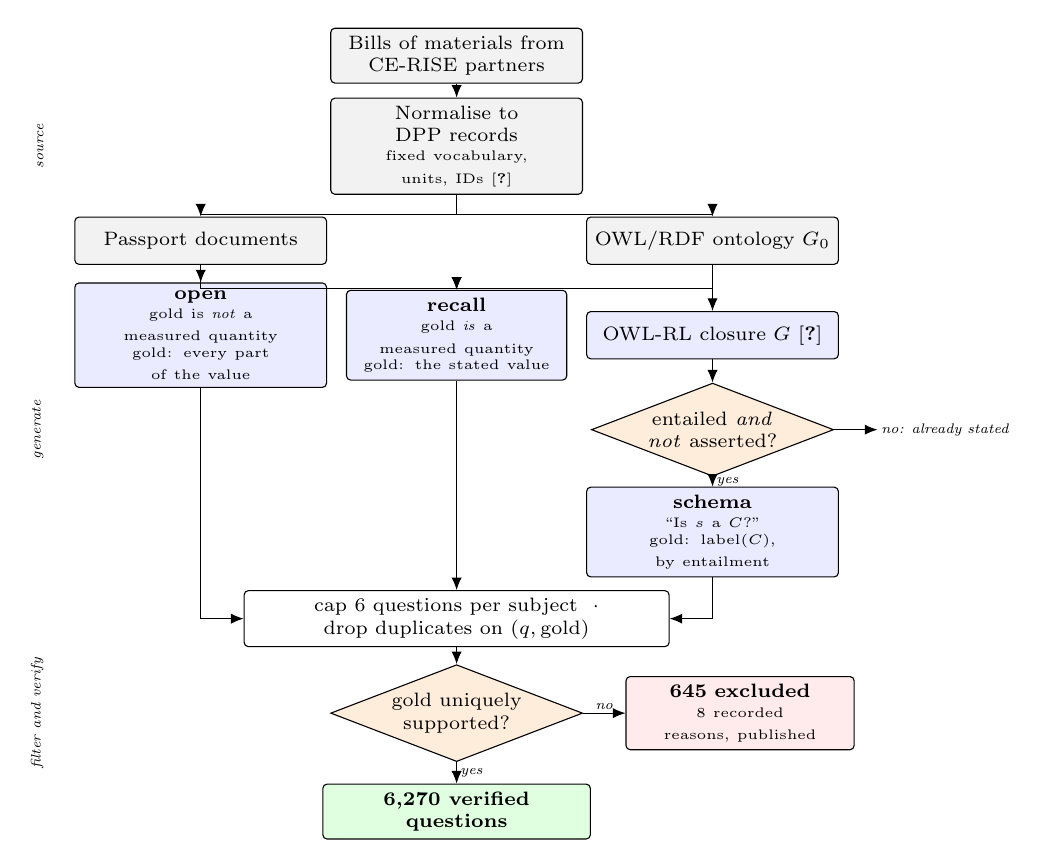
\begin{tikzpicture}[
  font=\scriptsize,
  % No hyphenation anywhere: the boxes are narrow and broken words
  % ("clo-sure", "veri-fied") read badly in a figure.
  every node/.append style={align=center,
    execute at begin node={\hyphenpenalty=10000\exhyphenpenalty=10000}},
  box/.style  ={draw,rounded corners=1.5pt,inner sep=2.8pt,
                minimum height=6mm,text width=30mm,fill=white},
  src/.style  ={box,fill=black!5},
  gen/.style  ={box,fill=blue!8},
  dec/.style  ={draw,diamond,aspect=2.6,inner sep=0pt,
                text width=19mm,fill=orange!14},
  res/.style  ={box,fill=green!12,font=\scriptsize\bfseries,text width=32mm},
  drop/.style ={box,fill=red!8,text width=27mm},
  ar/.style   ={-{Latex[length=1.6mm,width=1.3mm]},thin},
  lbl/.style  ={font=\tiny\itshape,inner sep=1.2pt}]

\def\xL{-3.25}   % left  track x
\def\xR{ 3.25}   % right track x

% ---- source --------------------------------------------------------------
\node[src] (bom)  at (0, 0)     {Bills of materials from\\ CE\nobreakdash-RISE partners};
\node[src] (norm) at (0,-1.15)  {Normalise to DPP records\\[-1pt]
                                 {\tiny fixed vocabulary, units, IDs~\cite{esfarealam2025synthdpp}}};

% ---- two renderings of the same product ----------------------------------
\node[src] (doc) at (\xL,-2.35) {Passport documents};
\node[src] (ont) at (\xR,-2.35) {OWL/RDF ontology $G_0$};

% ---- ontology track ------------------------------------------------------
\node[gen] (clo) at (\xR,-3.55) {OWL\nobreakdash-RL closure $G$~\cite{owlrl2012}};
\node[dec] (ent) at (\xR,-4.75) {entailed \emph{and}\\ \emph{not} asserted?};

% ---- generators ----------------------------------------------------------
\node[gen] (gopen) at (\xL,-3.55) {\textbf{open}\\[-1pt]
        {\tiny gold is \emph{not} a measured quantity}\\[-2pt]
        {\tiny gold: every part of the value}};
\node[gen,text width=26mm] (grec)  at (0,-3.55) {\textbf{recall}\\[-1pt]
        {\tiny gold \emph{is} a measured quantity}\\[-2pt]
        {\tiny gold: the stated value}};
\node[gen] (gsch)  at (\xR,-6.05) {\textbf{schema}\\[-1pt]
        {\tiny ``Is $s$ a $C$?''}\\[-2pt]
        {\tiny gold: $\mathrm{label}(C)$, by entailment}};

% ---- filters -------------------------------------------------------------
\node[box,text width=52mm] (filt) at (0,-7.15)
        {cap 6 questions per subject\ \ $\cdot$\ \ drop duplicates on $(q,\text{gold})$};
\node[dec] (ver)  at (0,-8.35) {gold uniquely\\ supported?};
\node[drop] (excl) at (3.6,-8.35) {\textbf{645 excluded}\\[-1pt]
        {\tiny 8 recorded reasons, published}};
\node[res] (fin)  at (0,-9.6) {6{,}270 verified questions};

% ---- edges ---------------------------------------------------------------
\draw[ar] (bom) -- (norm);
\draw[ar] (norm.south) -- ++(0,-0.25) -| (doc.north);
\draw[ar] (norm.south) -- ++(0,-0.25) -| (ont.north);

\draw[ar] (doc) -- (gopen);                           % no unit in gold
\draw[ar] (doc.south) -- ++(0,-0.3) -| (grec.north);  % unit in gold
\draw[ar] (ont.south) -- ++(0,-0.3) -| (grec.north);  % asserted triples
\draw[ar] (ont) -- (clo);
\draw[ar] (clo) -- (ent);
\draw[ar] (ent) -- node[lbl,right] {yes} (gsch);
\draw[ar] (ent.east) -- ++(0.55,0) node[lbl,above right,anchor=west]
          {no: already stated};

\draw[ar] (gopen.south) |- ($(filt.west)+(-0.0,0)$);
\draw[ar] (grec.south)  -- (filt.north);
\draw[ar] (gsch.south)  |- (filt.east);

\draw[ar] (filt) -- (ver);
\draw[ar] (ver)  -- node[lbl,above] {no}  (excl);
\draw[ar] (ver)  -- node[lbl,right] {yes} (fin);

% ---- stage labels --------------------------------------------------------
\node[lbl,anchor=south,rotate=90] at (-5.2,-1.15) {source};
\node[lbl,anchor=south,rotate=90] at (-5.2,-4.75) {generate};
\node[lbl,anchor=south,rotate=90] at (-5.2,-8.35) {filter and verify};
\end{tikzpicture}
}
\caption{\color{black}Automated question generation. Each product is rendered
twice, as a passport document and as an ontology individual, so the same record
can be questioned two ways. Only the schema branch computes anything: a question
is emitted where a type is entailed by the ontology but never asserted in it, so
its answer cannot be found by searching the record. \protect\newrev}
\label{fig:genflow}
\end{figure*}
\end{comment}



\subsection{Why a verified evaluation set}
\label{sec:verified}
A benchmark built from real product documentation contains questions whose
correct answer is not uniquely determined. A knowledge base may support two
conflicting statements about the same entity, a document label may be malformed, or the expected value may appear only as a placeholder. Scoring any system on such a question measures the benchmark rather than the system.
We therefore keep a question only when its answer is uniquely and atomically
supported by the evidence. The exclusion criteria are objective, applied without
looking at any system's output, and fixed in advance. \ExcludedRows{} rows are
removed under \ExcludedReasons{} recorded reasons, the largest groups being
conflicting knowledge-base evidence and malformed document labels. What remains
is \VerifiedN{} questions across \VerifiedDomains{} industrial domains.
The exclusions are published with the benchmark, so a reader who disagrees with
a criterion can recompute without it.

Table~\ref{tab:excl} lists the exclusion criteria and the number of questions removed by each. All criteria are properties of the source record and can be assessed without running any configuration, including conflicting relations, malformed labels, placeholder or non-unique gold values, unexpected lists, and classes not derivable by the reasoner. The latter illustrates why generation and filtering are separate stages: a well-formed question may still lack a uniquely determined answer.

\begin{table}[t]
\caption{Verified-subset filter. Every criterion is objective and is
applied before evaluation, without reference to any configuration's output.}
\label{tab:excl}
\centering\footnotesize
\setlength{\tabcolsep}{4pt}
\begin{tabular}{@{}>{\raggedright\arraybackslash}p{0.62\columnwidth}r@{}}
\toprule
criterion & removed \\
\midrule
entity carries two conflicting relations & 256 \\
document label malformed & 146 \\
gold not uniquely supported by the record & 94 \\
gold is a placeholder, not a value & 75 \\
gold is a list where one item is expected & 28 \\
record-level class not verifiable & 21 \\
class not derivable under entailment & 15 \\
document label ambiguous & 10 \\
\midrule
total removed & \ExcludedRows \\
retained & \VerifiedN \\
\bottomrule
\end{tabular}
\end{table}

\subsection{Configurations}
All four configurations are scored on the same \VerifiedN{} rows. The external
baselines are scored from their released outputs filtered to those rows, not
re-run.

\emph{LongCtx} places the record in a long-context language model.
\emph{LINC} and \emph{LogicLM} translate the question into a formal
representation and delegate to a solver. The fourth configuration adds two
things: it checks rule-governed questions against a machine-readable version of
the applicable constraints, and it withholds an answer when the combined
evidence is not sufficient to support one.

\textbf{Models.} LINC and Logic-LM are reasoning frameworks rather than
models, and each was originally evaluated over several language-model
backbones, so naming the framework does not by itself identify what was run.
The rows reported here are our own implementations of the two baseline strategies---a premise-and-goal chain for LINC~\cite{olausson2023linc} and classify-then-dispatch for Logic-LM~\cite{pan2023logiclm}---instantiated on a
common backbone rather than the model configurations reported in the original
papers, and they should not be read as reproductions of those papers' numbers.
For the implementations evaluated here the generation backbone is held fixed at
\GenModel{}, with \EmbedModel{} used for retrieval where retrieval applies.
Holding the backbone fixed is deliberate: it makes the differences in
Section~\ref{sec:results} attributable to how each configuration combines
evidence rather than to model capability. The cost of that control is that the
experiment does not establish whether the depth-dependent pattern persists,
narrows, or changes with frontier-scale models, and we include LINC and Logic-LM
as established neuro-symbolic strategies rather than as representatives of the
current frontier.

\subsection{The depth-aware configuration}
\label{sec:depthaware}
The fourth configuration combines three modules: a \emph{retrieval} module that locates evidence in the record, supporting depth-one and most depth-two questions; a \emph{memory} module that retains values established earlier in the session; and a \emph{reasoning} module that validates candidate answers against the machine-readable schema and applicable constraints required at depth three. Rather than forming a fixed pipeline, these modules are engaged on demand according to \revg{the evidence available for the question}, and an answer is returned only when their combined evidence is sufficient; otherwise, the configuration abstains. This selective coordination defines the \emph{depth-aware} approach, while the internal design and individual contributions of the modules are reported separately.

\revg{The benchmark's fusion-depth label is not supplied to the configuration
at inference time: the request contains the question, product identifier and
session state, but no depth field. The controller chooses memory, symbolic,
retrieval or combined processing from the memory-match score, symbolic
applicability and retrieval score. The gold label is used only after answering
to stratify evaluation. Thus, \emph{depth-aware} denotes evidence-dependent
routing rather than oracle access to the benchmark label. \revg{The three
baselines, by contrast, are told the question type in their prompt, so what
label information exists in this comparison favours them rather than the
depth-aware configuration.}}


%The fourth configuration combines three modules. A \emph{retrieval} module locates evidence in the record, which is sufficient at depth one and does most of the work at depth two. A \emph{memory} module holds values established earlier in a session, contributing a source the document itself does not contain. A \emph{reasoning} module checks a candidate answer against the machine-readable schema and the applicable constraints, which is what depth three requires.

%They are not run as a fixed pipeline. Each question engages only the modules its depth needs, and an answer is released only when their combined output supports it; otherwise the configuration abstains. That coordination is what \emph{depth-aware} refers to. The internal design of each module, and the contribution each makes, are reported separately.

Algorithm~\ref{alg:depth} summarizes the control flow. A question first consults base memory for values established earlier in the session, while unresolved information is retrieved from passport documents and the ontology through external memory. The reasoner is invoked only when the required fact is not stated in the record, deriving it from the schema when possible. The resulting evidence is assembled into a single context from which the language model generates the answer. If any required component is missing, the configuration abstains rather than guessing, reducing coverage under insufficient evidence as evaluated in Section~\ref{sec:off}.



%\rev{Algorithm~\ref{alg:depth} states the control flow at the level the comparison requires. A question first consults base memory, which holds values already established for the product in this session. Whatever remains unresolved is sent to external memory, the retrieval step over passport documents and the ontology. The reasoner is then invoked only when the question needs a fact that the record does not state, and it either derives that fact from the schema or reports that it cannot. The three outputs are assembled into a single context, and the language model is asked to compose an answer from that context alone rather than from its own knowledge. The final gate is the one that matters for the results in Section~\ref{sec:off}: if a required component is missing, the configuration returns an abstention instead of an answer, so a low-evidence question lowers coverage rather than producing a confident guess.}

\begin{comment}
\begin{figure}[t]
\normalcolor
\centering
\resizebox{0.86\columnwidth}{!}{% Flowchart: depth-aware answering. Deliberately stops at the level the
% comparison requires; module internals are not shown.
%
% Requires in the preamble of the including document:
%   \usepackage{tikz}
%   \usetikzlibrary{shapes.geometric,arrows.meta,positioning,calc}
%
% Bypass edges run down the LEFT margin and the abstain edge to the RIGHT, so
% the two never cross.
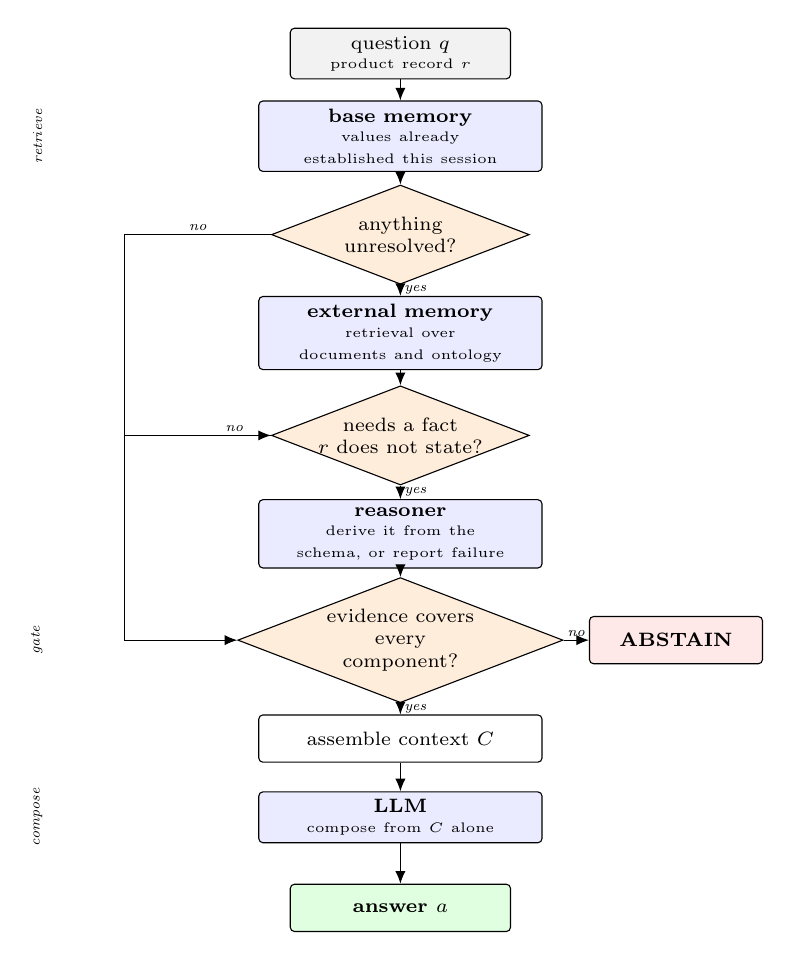
\begin{tikzpicture}[
  font=\scriptsize,
  every node/.append style={align=center,
    execute at begin node={\hyphenpenalty=10000\exhyphenpenalty=10000}},
  box/.style  ={draw,rounded corners=1.5pt,inner sep=2.8pt,
                minimum height=6mm,text width=34mm,fill=white},
  mod/.style  ={box,fill=blue!8},
  dec/.style  ={draw,diamond,aspect=2.6,inner sep=0pt,
                text width=21mm,fill=orange!14},
  io/.style   ={box,fill=black!5,text width=26mm},
  good/.style ={box,fill=green!12,font=\scriptsize\bfseries,text width=26mm},
  stop/.style ={box,fill=red!9,font=\scriptsize\bfseries,text width=20mm},
  ar/.style   ={-{Latex[length=1.6mm,width=1.3mm]},thin},
  lbl/.style  ={font=\tiny\itshape,inner sep=1.2pt}]

\def\BY{-3.5}   % x of the bypass lane, left of everything

\node[io]   (q)     at (0, 0)    {question $q$\\[-1pt]{\tiny product record $r$}};
\node[mod]  (bm)    at (0,-1.05) {\textbf{base memory}\\[-1pt]
        {\tiny values already established this session}};
\node[dec]  (unres) at (0,-2.30) {anything\\ unresolved?};
\node[mod]  (em)    at (0,-3.55) {\textbf{external memory}\\[-1pt]
        {\tiny retrieval over documents and ontology}};
\node[dec]  (needs) at (0,-4.85) {needs a fact\\ $r$ does not state?};
\node[mod]  (rea)   at (0,-6.10) {\textbf{reasoner}\\[-1pt]
        {\tiny derive it from the schema, or report failure}};
\node[dec]  (gate)  at (0,-7.45) {evidence covers\\ every component?};
\node[stop] (abst)  at (3.5,-7.45) {ABSTAIN};
\node[box]  (ctx)   at (0,-8.70) {assemble context $C$};
\node[mod]  (llm)   at (0,-9.70) {\textbf{LLM}\\[-1pt]
        {\tiny compose from $C$ alone}};
\node[good] (ans)   at (0,-10.85) {answer $a$};

% ---- straight-through path ----------------------------------------------
\draw[ar] (q)     -- (bm);
\draw[ar] (bm)    -- (unres);
\draw[ar] (unres) -- node[lbl,right] {yes} (em);
\draw[ar] (em)    -- (needs);
\draw[ar] (needs) -- node[lbl,right] {yes} (rea);
\draw[ar] (rea)   -- (gate);
\draw[ar] (gate)  -- node[lbl,right] {yes} (ctx);
\draw[ar] (ctx)   -- (llm);
\draw[ar] (llm)   -- (ans);

% ---- bypasses: a module runs only when the question needs it -------------
\draw[ar] (unres.west) -- node[lbl,above] {no} (\BY,-2.30) -- (\BY,-4.85)
          -- (needs.west);
\draw[ar] (needs.west) -- node[lbl,above,pos=0.25] {no} (\BY,-4.85)
          -- (\BY,-7.45) -- (gate.west);

% ---- abstain, on the opposite side --------------------------------------
\draw[ar] (gate) -- node[lbl,above] {no} (abst);

\node[lbl,anchor=south,rotate=90] at (-4.5,-1.05) {retrieve};
\node[lbl,anchor=south,rotate=90] at (-4.5,-7.45) {gate};
\node[lbl,anchor=south,rotate=90] at (-4.5,-9.70) {compose};
\end{tikzpicture}
}
\caption{\color{black}Depth-aware answering. A module runs only when the
question needs it, so the two \emph{no} branches skip work rather than perform
it. The gate sits before generation, not after: a question whose evidence is
incomplete is withheld instead of answered. \protect\newrev}
\label{fig:depthflow}
\end{figure}
\end{comment}

\vspace{9pt}
\hrule
\vspace{-8pt}
\begin{algorithm}[h]
\vspace{3pt}
\hrule
\vspace{1pt}
\normalcolor  % floats are typeset later; do not inherit \hl's colour state
\caption{\color{black}Depth-aware answering. 
%Pseudocode for Fig.~\ref{fig:depthflow}; 
Modules are engaged on demand, and the answer is gated on the evidence actually assembled. 
}
\label{alg:depth}
\begin{pseudo}
\vspace{5pt}
\item[] \kw{Input:} question $q$; product record $r$; session state $M$
        \revg{\cmt{no depth label}}
\item[] \kw{Output:} answer $a$, or \pr{Abstain}
\item $E \gets \pr{BaseMemory}(q,M)$ \cmt{values already established}
\item $N \gets \pr{Unresolved}(q,E)$
\item \kw{if} $N \neq \emptyset$ \kw{then}
\item[] \IND $E \gets E \cup \pr{ExternalMemory}(N,r)$
        \cmt{retrieve over documents and ontology}
\item \kw{if} $\revg{\pr{SymbolicApplicable}(q,E,r)}$ \kw{then}
\item[] \IND $E \gets E \cup \pr{Reason}(q,E)$
        \revg{\cmt{applicability inferred; derive or fail}}
\item \kw{if} $E$ does not cover every component $q$ asks for \kw{then}
\item[] \IND \kw{return} \pr{Abstain} \cmt{lower coverage, do not guess}
\item $C \gets \pr{AssembleContext}(E)$
\item $a \gets \pr{LLM}(q,C)$ \cmt{compose from $C$ alone}
\item \kw{return} $a$
\end{pseudo}
\vspace{1pt}
\hrule
\end{algorithm}
% =====================================================================
\section{Results}
\label{sec:results}
% =====================================================================

\subsection{A trade-off across fusion depth}

Table~\ref{tab:main} and Fig.~\ref{fig:bytype} report accuracy at each fusion
depth.
The overall scores make the three systems look similar: they are
separated by only \SpreadOverall{} percentage points. Grouping the same
questions by fusion depth gives a different result.

\begin{table}[t]
\caption{Accuracy on the same \VerifiedN{} verified questions, grouped by fusion
depth. Best baseline per column in bold. The three published systems are within
\SpreadOverall{} points overall, but no system is best at more than one depth.}
\label{tab:main}
\centering\footnotesize
\setlength{\tabcolsep}{4.5pt}
\begin{tabular}{lcccc}
\toprule
& \multicolumn{3}{c}{by fusion depth} & \\
\cmidrule(lr){2-4}
configuration & recall & open & rule & overall \\
\midrule
LongCtx & \AccLongCtxRecall & \AccLongCtxOpen & \AccLongCtxLogic & \AccLongCtx \\
LINC & \AccLINCRecall & \AccLINCOpen & \textbf{\AccLINCLogic} & \AccLINC \\
LogicLM & \textbf{\AccLogicLMRecall} & \textbf{\AccLogicLMOpen} & \AccLogicLMLogic & \AccLogicLM \\
\midrule
headroom to ceiling & \HeadroomRecall & \HeadroomOpen & \HeadroomLogic & \\
\midrule
fused + selective & \AccSysRecall & \AccSysOpen & \AccSysLogic & \AccSys \\
\bottomrule
\end{tabular}
\end{table}





LongCtx and LogicLM are almost perfect on recall questions, reaching
\AccLongCtxRecall\% and \AccLogicLMRecall\%, respectively. Their accuracy falls
to \AccLongCtxLogic\% and \AccLogicLMLogic\% on rule-governed questions. At
this depth, finding the product value is not enough; the answer also requires
that value to be combined with the schema rules that classify it, and is
therefore not present in the retrieved text.

\begin{figure}[h]
\centering
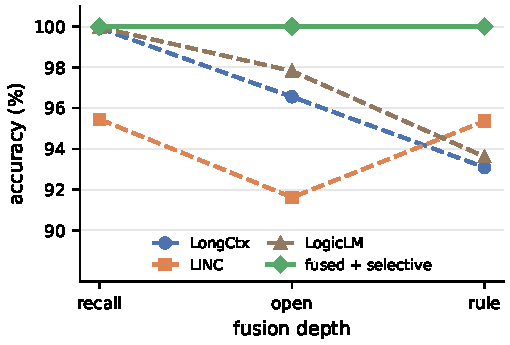
\includegraphics[width=0.85\columnwidth]{by_type.pdf}
\caption{Accuracy across fusion depth. Long-context and LogicLM are strongest
on questions that need little fusion, while LINC improves on rule-governed
questions but loses accuracy at shallower depths.}
\label{fig:bytype}
\end{figure}

LINC shows the opposite pattern. It is the strongest baseline on rule-governed
questions at \AccLINCLogic\%, but the weakest on recall at
\AccLINCRecall\% and on open questions at \AccLINCOpen\%. LINC translates
questions into a formal representation before reasoning. This helps when a
formal rule must be applied, but adds machinery to questions that can be
answered from the record more directly.

The result is therefore a trade-off rather than a single ranking. A system that
is strongest at one fusion depth can be weaker at another. We define
\emph{headroom} as the difference between the best baseline accuracy and a
perfect score. It increases from \HeadroomRecall{} points for recall questions
to \HeadroomOpen{} for open questions and \HeadroomLogic{} for rule-governed
questions. \revg{On this benchmark, most of the observed headroom is therefore
at the deeper fusion levels rather than at simple value retrieval; this
empirical ordering is not part of the definition of depth.}

\revg{The high absolute scores should be interpreted in light of the benchmark
design: the verified subset has uniquely supported answers, three fixed
question forms, and depth-three class-membership entailments over subclass
chains of one to three steps. It excludes temporal or numerical rules,
negation and conflicting-rule resolution. The schema validator is deliberately
matched to this task, and substring scoring can also make absolute accuracy
optimistic even though it is applied identically to all configurations. The
100\% is therefore a ceiling result for this controlled rule
fragment, not evidence that general depth-three reasoning is solved; the main
result is the comparison between strategies across evidence regimes. The
separate Open Food Facts arm measures a different setting: it reaches
\OffAcc\% \emph{decision} accuracy on an unseen public schema while answering
\OffCoverage\% of queries. Because a justified abstention is a correct decision
there, this figure should not be read as ordinary answer accuracy at full
coverage.}

Table~\ref{tab:domain} shows the same pattern across the three industrial
domains. Battery has the largest share of rule-governed questions
(\ShareMostRule\%) and the lowest average baseline accuracy. Viessmann(Heatpump Domain) has
the smallest share (\ShareLeastRule\%) and the highest average baseline
accuracy, with Lexmark(Printer Domain) between them. This suggests that domains containing
more rule-governed questions are harder for the baseline approaches. Since
we evaluate only \VerifiedDomains{} domains, we report this as an observed
pattern rather than a statistical correlation.

\begin{table}[t]
\caption{Accuracy by industrial domain, ordered by the share of rule-governed questions each domain carries. Baseline accuracy falls as that share rises; the ordering is recomputed from the artifacts on every build.}
\label{tab:domain}
\centering\footnotesize
\setlength{\tabcolsep}{5pt}
\begin{tabular}{lccc}
\toprule
configuration & battery & lexmark & viessmann \\
\midrule
rule-governed share (\%) & 53.9 & 45.7 & 33.3 \\
\midrule
LongCtx & 93.70 & 96.82 & 97.75 \\
LINC & 93.77 & 92.56 & 97.60 \\
LogicLM & 94.25 & 97.56 & 97.79 \\
\midrule
fused + selective & 100.00 & 100.00 & 100.00 \\
\bottomrule
\end{tabular}
\end{table}



\subsection{Selective fusion avoids the observed trade-off}

The previous result suggests a simple alternative: use symbolic reasoning only
for questions that need it, rather than applying the same reasoning strategy to
every question. Average accuracy alone cannot show whether this helps without
hurting other cases. A system may gain accuracy on some questions while losing
it on others.

Because all configurations are evaluated on the same \VerifiedN{} questions,
we can compare them question by question. We call this a \emph{paired
comparison}. Table~\ref{tab:mcnemar} reports the disagreements: cases where
only the depth-aware configuration is correct, and cases where only the
baseline is correct.



LongCtx, LINC, and LogicLM leave \ErrLongCtx{}, \ErrLINC{}, and
\ErrLogicLM{} errors, respectively, while the depth-aware configuration leaves
\ErrSys{} on this verified set. More importantly, the right-hand column of
Table~\ref{tab:mcnemar} is zero for every comparison. In other words, there is
no question in this set that a baseline answers correctly and the depth-aware
configuration answers incorrectly.

\begin{table}[h]
\caption{Paired disagreements between each baseline and the depth-aware
configuration. The baseline-only column is zero in all three comparisons.}
\label{tab:mcnemar}
\centering\footnotesize
\setlength{\tabcolsep}{5pt}
\begin{tabular}{lcc}
\toprule
baseline & fused-only correct & baseline-only correct \\
\midrule
LongCtx & \DiscLongCtxSysOnly & \DiscLongCtxBaseOnly \\
LINC & \DiscLINCSysOnly & \DiscLINCBaseOnly \\
LogicLM & \DiscLogicLMSysOnly & \DiscLogicLMBaseOnly \\
\bottomrule
\end{tabular}
\end{table}

We use the exact McNemar test to check whether the improvement could reasonably
be explained by chance. The test considers only questions on which the two
configurations disagree. For example, the depth-aware configuration corrects
\DiscLogicLMSysOnly{} LogicLM errors, while LogicLM corrects none of its
errors. All three comparisons give $p < 10^{-\McnExp}$, meaning that such
one-sided differences would be extremely unlikely if the two configurations
performed equally well. More importantly, the paired counts show the practical
result directly: on this set, the depth-aware configuration corrects baseline
errors without losing any question that a baseline answers correctly.


\subsection{Knowing when the evidence is insufficient}
\label{sec:off}

The verified benchmark contains only questions with a unique supported answer.
Real product databases are less complete. A reliable system must therefore know
not only \emph{what} to answer, but also when the available evidence is too weak
to support an answer.

We test this on \OffN{} queries from Open Food Facts~\cite{openfoodfacts}, a
public product database with a different schema, different field names, and
substantial missing data. The purpose is to test whether the
configuration can transfer to a new data source and avoid guessing when
information is missing.

We first measure \emph{decision accuracy}. A decision is correct when the
system gives the right answer when enough evidence exists, or abstains when it
does not. The configuration reaches \OffAcc\% decision accuracy, with a Wilson
95\% confidence interval of \OffAccLo--\OffAccHi\%, while answering
\OffCoverage\% of all queries. Coverage therefore tells us how often the
system chooses to answer rather than abstain.

We also check whether its confidence is useful for making that choice. Expected
calibration error (ECE) measures the gap between stated confidence and observed
correctness; lower is better. The system reaches an ECE of \OffEce{}. Its
risk--coverage score, \OffAurc{}, summarizes how error changes as more queries
are answered. When the system abstains, it is almost always justified:
abstention precision is \OffAbstainPrec{} at recall \OffAbstainRec{}.

\begin{table}[t]
\caption{Public-schema arm by query type. Where the underlying fields are sparsely populated there is little to combine, and the system lowers coverage rather than guessing.}
\label{tab:off}
\centering\footnotesize
\setlength{\tabcolsep}{4.5pt}
\begin{tabular}{lcccc}
\toprule
query type & $n$ & accuracy & coverage & ECE \\
\midrule
nutrition & 1450 & 100.00 & 69.6 & 0.004 \\
missingness & 367 & 92.92 & 100.0 & 0.071 \\
attribute & 1146 & 99.83 & 99.8 & 0.002 \\
sustainability & 1039 & 91.92 & 38.0 & 0.060 \\
fairness & 19 & 100.00 & 100.0 & 0.000 \\
\midrule
all & 4021 & 97.21 & 73.0 & 0.021 \\
\bottomrule
\end{tabular}
\end{table}


Table~\ref{tab:off} shows where this behaviour comes from. Questions about
stated nutrition values and product attributes are answered almost perfectly,
showing that simple retrieval transfers well to the new schema. The hardest
category is \OffHardestType{}, with \OffHardestAcc\% accuracy, and the system
answers only \OffHardestCoverage\% of these queries.

These questions often depend on fields that are missing or inconsistently
defined. Instead of forcing an answer, the system lowers its coverage and
abstains more often. Its ECE also rises to \OffEceHardest{} on this subset,
showing that the same questions are both harder and less certain. This is the
behaviour the experiment is designed to test: when the evidence becomes weak,
the system should answer less often rather than guess.
% =====================================================================
\section{What the Results Show and Their Limits}
\label{sec:limits}
% =====================================================================

The results support three main conclusions, but they also have clear limits.
\textit{First}, the trade-off across fusion depth is observed for three established strategies on this benchmark. The systems are close in overall accuracy but behave
differently once the questions are separated by depth. This shows that a single
accuracy score can hide differences that matter in practice. It does not show
that every possible uniform strategy must follow the same pattern.
\textit{Second}, the verified benchmark contains only questions with a unique supported
answer. Its rule-governed questions are also checked against machine-readable
constraints. A configuration that routes these questions to symbolic validation
is therefore expected to perform strongly. The result shows that the ceiling is
reachable on this verified set and that the baselines do not reach it. It does
not make a claim about the \ExcludedRows{} excluded questions. 

We publish those
rows and their exclusion reasons so this boundary is explicit.

\revg{The rule-governed subset carries a genuine \emph{benchmark--method
circularity}, which we state rather than qualify. Its gold answers are defined
by OWL-RL entailment over the domain ontology, and the depth-aware
configuration's symbolic layer computes that same closure. The overlap is not
partial: the symbolic layer fired on \SymFired{} of the \NLogic{} rule-governed
questions, that is \SymFiredPct\%, and was correct on \SymFiredAcc\% of the
questions where it fired. Depth-three accuracy is therefore a consistency check
between two applications of the same entailment procedure, not a measurement of
reasoning ability, and it should be read that way. What the circularity does
\emph{not} do is contaminate the comparison itself: questions, depths and gold
answers are fixed without consulting any system's output, and all four
configurations are scored on identical items. The ceiling result applies to the
evaluated entailment regime, not to unseen ontologies or rule languages;
held-out schemas and independently authored questions remain future work. The Open Food Facts evaluation partly addresses
schema transfer by testing \OffN{} queries from a public database with different
field names and substantial missingness. It supports generalisation of retrieval
and selective answering, but it is not a held-out OWL-RL entailment benchmark
and therefore does not by itself remove the circularity concern for depth
three.}

\revg{Because the concern is confined to one class, it can be removed rather
than only acknowledged. Excluding the rule-governed questions entirely leaves
\NoRuleN{} questions whose gold answers are copied from the source record and
never derived, so no generator--solver overlap is possible. On that subset the
depth-aware configuration still corrects \NoRuleDiscLongCtx{},
\NoRuleDiscLINC{} and \NoRuleDiscLogicLM{} errors made by LongCtx, LINC and
LogicLM respectively, while losing no question that any of them answers
correctly. Accuracy on that subset is \NoRuleLongCtx\%,
\NoRuleLINC\% and \NoRuleLogicLM\% for the three baselines against
\NoRuleSys\%. The margin is much smaller than on the full set, as it should be
once the aligned class is removed, but the one-sided direction of the result
does not depend on that class.}

The paired comparison gives a similarly limited conclusion. On these
\VerifiedN{} questions, the depth-aware configuration corrects baseline errors
without losing any question that a baseline answers correctly. This is strong
evidence for this benchmark, but it is not a guarantee that the same one-sided
result will hold on unseen data.

The three depths are a controlled operational taxonomy, not a universal
classification standard. Deployed systems may require evidence beyond this
benchmark: temporal reasoning, numerical computation against a
threshold, aggregation across records, resolution of conflicting sources, and
evidence in other modalities. The underlying principle is domain independent---
a question can be classified by whether its answer is stated, assembled, or
derived---but the prevalence and form of these requirements need not be
constant across industries, and our own domains already differ, carrying
\ShareMostRule\% and \ShareLeastRule\% rule-governed questions at the extremes.
We thus claim reproducibility of the classification within the evaluated
schemas, not completeness or universality across industrial fields.

The questions also use a narrow set of surface forms. Every item is either
``What is the $p$ of $s$?'', ``According to $d$, what is the $f$?'', or ``Is $s$
a $C$?''. There are no existential, temporal, quantitative or negated forms and
no paraphrase variation, so the benchmark varies evidence combination while
holding phrasing almost constant. That is deliberate, because it is what keeps
every gold answer mechanically derivable, but it means these results say nothing
about robustness to how a question is worded. Widening the templates would
require regenerating the benchmark and re-running every configuration, so we
report the limitation rather than partly addressing it.

Relatedly, on the document side the depth-one and depth-two labels are
assigned by a surface test on the gold value rather than by a semantic
judgement, as Section~\ref{sec:gen} states. The test is reproducible and it
tracks difficulty, but a different operationalisation would move some questions
across the boundary.

The two evaluation settings also measure different abilities. The verified set
tests accuracy when a supported answer exists. The Open Food Facts evaluation
tests whether the system can also recognise when the available evidence is not
enough. This is why coverage and calibration are reported there. Whether
\OffCoverage\% coverage is acceptable depends on the cost of withholding an
answer in a particular application.

Finally, this paper compares complete configurations. It does not isolate the
effect of symbolic validation from the effect of selective abstention. That
requires an ablation study, which is reported separately.


% =====================================================================
\section{Conclusion}
% =====================================================================

\revg{Question answering over product records requires different evidence operations,
from retrieving a stated value to deriving a schema-mediated answer.} When we
group the same questions by fusion depth,
the three established strategies that appear similar in overall accuracy show very
different strengths. Long-context and LogicLM perform best on shallower
questions, while LINC performs better when record evidence must be combined
with an external rule. A single accuracy score hides this trade-off.

The results also show why a depth-aware strategy can be useful. Simple recall
questions need little additional reasoning, while rule-governed questions leave
more room for improvement. Applying symbolic validation only when needed
avoids the loss seen when formal reasoning is applied uniformly. On the verified
set, this configuration reaches the ceiling without losing any question that a
baseline answers correctly. On the public-database evaluation, it also reduces
coverage when the available evidence is too weak to support an answer.

Although our experiments focus on DPP, the underlying
idea is broader. Other applications also combine stored records with external
rules, including clinical guidelines, financial reporting, and safety
certification. In such settings, evaluating systems by how much evidence a
question requires may reveal differences that a single overall accuracy score
cannot show.
Future work will extend the fusion-depth framework to more complex evidence requirements, including temporal and numerical reasoning, aggregation across multiple records, and conflicting or multimodal evidence.


\section*{Reproducibility}

The verified set, its exclusion records with reasons, the per-question outputs
of all four configurations, and the public-database evaluation summary are
released at \url{https://github.com/aeturzo/dpp-qa-fusion-depth_forAIPMV}. Every number
in this paper is generated from those files, and the released
\texttt{verify\_all.py} re-derives all of them and fails if any disagrees with
the value printed here; none is transcribed by hand. The same repository
reports what changes under stricter grading of the question classes.

\section*{Acknowledgment}
This work has received funding from the European Union (EU) under the Horizon 2020 Research and Innovation Programme through Grant Agreement No. 101092281 (CE-RISE) and from the European Health and Digital Executive Agency under Grant Agreement No. 101226256 (3D-CIRCULAR).
Views and opinions expressed are however those of the
author(s) only and do not necessarily reflect those of the
European Union or Horizon Europe. Neither the EU nor the granting authority can be held responsible for
them.
This work was also supported in part by the Norwegian Research
Council under Grant 336617 (REWARD project) and Grant 355434 (SecondPass project).

%This work was supported by the CE-RISE project, which has received funding from the European Union's Horizon Europe research and innovation programme under grant agreement No.\ 101092281. Views and opinions expressed are those of the authors only and do not necessarily reflect those of the European Union or the granting authority, neither of which can be held responsible for them.

\section*{Generative AI Disclosure}
Generative AI assistants (Anthropic Claude; OpenAI Codex) were used for language
editing, \LaTeX{} preparation, and the reproducibility tooling released with this
paper. They were not used to produce, select, or analyse experimental results:
every figure reported here is generated from locked evaluation artifacts by the
released scripts. 
%The authors verified every claim, reference, and numerical value against those artifacts and are solely responsible for the content.

\bibliographystyle{IEEEtran}
\bibliography{refs}

\end{document}
